\section{Calculations}

For each \gls{WTM} at each wind velocity, the data collected from the wind tunnel consisted of a time series of voltages corresponding to the measured drag force and the measured wind velocity, as well as the points in time when the first zero measurement and the second zero measurement were conducted and when the 60 \si{\s} drag measurement started. Using Matlab, this data was treated.

The force plate was assumed to drift linearly. Thus, using the two zero measurement values, a linear function approximating the drift was created. The part of this linear function corresponding to the 60 \si{\s} where the force measurement was conducted, was extracted, as seen in figure \ref{Fig:driftAdjust}. For each measured force in the time series, the corresponding drift was subtracted. After, the average drag force over the time series was calculated, as well as the variance and standard deviation. 

\begin{figure}
    \centering
    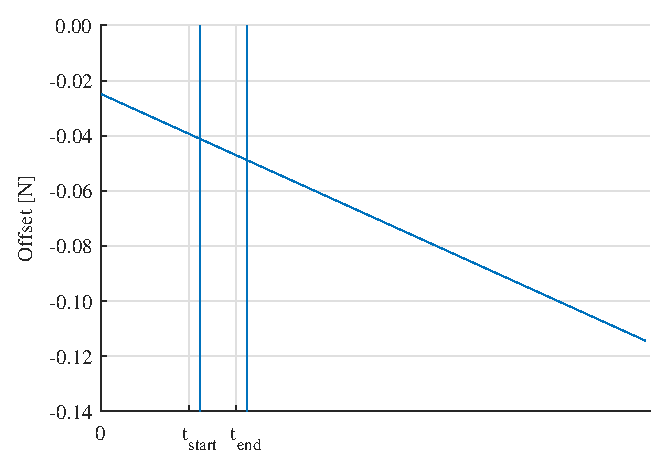
\includegraphics[width=0.5\textwidth]{0_Images/DriftDown.eps}    
    \caption{The approximated drift between the two zero measurements. $t_{start}$ indicated where the 60 \si{s} measurement started, and $t_{end}$ indicated where the measurement ended.}
    \label{Fig:driftAdjust}
\end{figure}

In the same matter, the drift was subtracted and the average drag force was calculated for the measurements that were conducted using only the base and the tower, for each of the different wind velocities. These average drag forces were then subtracted from the averages drag forces calculated earlier for all the different \gls{WTM}s, so that what remains is only the drag on the disks or the turbine blades, excluding the towers and the base. 
%the final drag force represented only

Finally, this calculated drag was divided by three, so as to only consider the drag on one disk or one set of rotating blades. This force was further used in calculating the drag coefficient, using equation \ref{Eq:Cd}, together with the total swiping area of the rotating turbine model, being $\pi r^2$.

Another value collected as part of the measurement data was the average temperature during the 60 \si{\s} of measuring. This was used to decide on the appropriate value for the air density, $\rho$, and air dynamic viscosity, $\mu$, when calculating the drag coefficient and the Reynolds number. However, the temperature only varied between about 20\degree C and 23\degree C. Since this variation is fairly small, it was assumed to not have any significant impact on the resulting drag.

\FloatBarrier

%Removing the towers: 
%\cite{Aubrun2019} concluded that the discrepancy in rod fixation and distance between wall and disc center can generate different wake downwasg that might explain differences. 